\documentclass{standalone}
\usepackage{tikz}
\usepackage{caption}
\usepackage{subcaption}
\usepackage{helvet}
\usepackage{adjustbox}
\renewcommand{\familydefault}{\sfdefault}
\usetikzlibrary{
  positioning, calc, shapes.geometric, shapes.multipart, 
	shapes, arrows.meta, arrows, 
	decorations.markings, external, trees}

% Arrow style:
\tikzset{
    Arrow/.style = {
        thick, 
        decoration={
            markings,
            mark=at position 1 with {
                \arrow[thick, #1]{latex}
                }
            }, 
        shorten >= 3pt, 
        preaction = {decorate}
    },
    Arrow/.default={black}
}
% Text node
\tikzset{
Node/.style={
  text width=1cm,
  align=center,
  }
}
% Colors
\definecolor{aFill}{HTML}{2980b9}
\definecolor{yFill}{HTML}{ee5253}
\definecolor{uFill}{HTML}{bdc3c7}
\begin{document}
\begin{adjustbox}{width=20cm, height=12cm, keepaspectratio}
  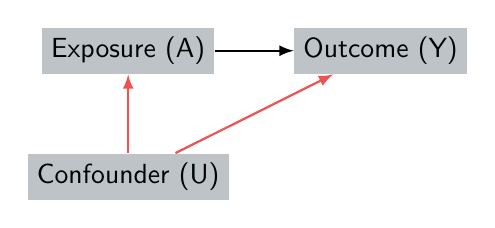
\begin{tikzpicture}
    \node [fill=uFill, align=center](U) {Confounder (U)};
    \node[fill=uFill, above=1cm of U] (A) {Exposure (A)};
    \node[fill=uFill, right=of A] (Y) {Outcome (Y)};
    \draw [Arrow=yFill, color=yFill] (U) to (A);
    \draw [Arrow=yFill, color=yFill] (U) to (Y);
    \draw [Arrow] (A) to (Y);
  \end{tikzpicture}
\end{adjustbox}
\end{document}